\documentclass{beamer}
\usetheme{boadilla}


\usepackage{amsmath,amssymb,amsthm} 
\usepackage{caption}
\usepackage{gensymb}
\usepackage{preview}
\usepackage{bm}
\usepackage{mathtools}
\usepackage{hyperref} 
\usepackage{fancyhdr}
\usepackage{indentfirst}
\usepackage{tablefootnote}
%\usepackage{cmbright}



\title{Theory Testing Using Mixtures and EM with our Buddies Imai and Tingley}
\subtitle{Machine Learning: Module 1}
\author{Sean Norton; Simon Hoellerbauer}
\begin{document}
\begin{frame}
	\titlepage
\end{frame}

\begin{frame}
\frametitle{Rationale}
Remember the general form of the mixture distribution where distributional forms can be different?
	\begin{align}
	p(x) = \sum_{k=1}^{K} \pi_k p (x | z_i = k, \theta)
	\end{align}
Well, today, we are going to treat the different mixing distributions as different statistical models that could have produced our observations (designated as $x$ here, but soon we will use $x$ for covariates and the more traditional---for us---$y$ for outcomes).
\end{frame}


\begin{frame}
\frametitle{Mixtures of Models: Data Generating Process}
We assume the following data generating process:
\begin{align}
	Y_i|X_i, Z_i \sim f_{Z_i}(Y_i|X_i, \theta_{Z_i})
\end{align}
Where $Y_i$ denotes the outcome for observation $i$, $X_I$ denotes the covariates for observation $i$, and $Z_i$ denotes the model $1-M$ that produced observation $i$. In other words, if we knew $Z_i$, we could tell you from which model $Y_I$ was drawn. Note that $\theta$ has a $Z_i$ subscript---a different set of $\theta$'s can belong to each model (or mixing distribution $m$). This also implies, of course, that the covariate set $X_i$ belong to observation $i$ does not have to be the same for each model. 
\end{frame}

\begin{frame}
\frametitle{Observed-Data Likelihood}
As usual, we assume conditional independence given covariates and the latent variable. This allows us to form the following observed-data likelihood function (where $Z$ has been integrated out):
\begin{align}
	L_{obs}(\Theta,\Pi|\{X_i, Y_i\}^N_{i=1}) = \prod^N_{i=1}\bigg\{\sum^M_{m=1}\pi_m f_m(Y_i|X_i, \theta_m) \bigg\}
\end{align}
Where the sum of all $\pi_m$ is 1 (because it is a distribution), $\Theta$ is the set of all $\theta$'s for all M theories (distributions/models), and $\Pi$ is the set of all $\pi$'s for all M theories (distributions/models).

This equation is important because it shows us that we can think of this model as weighting the various theories for each observation $i$
\end{frame}

\begin{frame}
\frametitle{Important Excursus: \textit{Theory-Predicting Variables}}
Being astute statisticians and wise mathematicians and amazing social scientists, it may come as no surprise, given the previous slide, that we can try to see if any variables influence the probability that an observation belongs to a certain model, which Imai and Tingley name a \textit{theory-predicting variables} and term as $W_i$. We then make the probability that the observation $i$ a function of $W_i$ and some parameters $\phi$:
\begin{align}
	Pr(Z_i=m|W_i) = \pi_m(W_i, \phi_m)
\end{align}
\color{red}
This is really, really cool, y'all.
\end{frame}

\begin{frame}
\frametitle{Let's Do Some EM-ing: Complete-Data Log-Likelihood}
We need the complete data log-likelihood to make applying the EM algorithm as straightforward as it can be:
\begin{align}
l_{com}(\Theta, \Pi|\{X_i, Y_i, Z_i\}^N_{i=1}) = \sum_{i=1}^{N}\sum_{m=i}^{M}\bigg(\log\pi_m + \log f_m(Y_i|X_i, \theta_m) \bigg)^{z_m}
\end{align}
Note that Imai and Tingley put the indicator function out in front, but it is the same thing as putting it in the exponent.
\end{frame}   

\begin{frame}
\frametitle{Let's Do Some EM-ing: The E-Step}
First, we must initialize all our parameters, so pick some $\Theta^{old}$ and some $\Pi^{old}$.

In this version of the E-step, we take the expectation of the complete-data log-likelihood w.r.t the posterior probabilities of the latent variable $Z_i$, such that
\begin{align}
	\mathbb{E}_{Z_i|\Theta^{old},\Pi^{old}, \{X_i, Y_i, Z_i\}^N_{i=1}} = 
	\sum_{i=1}^{N}\sum_{m=i}^{M} \zeta^{old}_{i,m} \bigg(\log\pi_m + \log f_m(Y_i|X_i, \theta_m) \bigg)
\end{align}
Where 
\begin{align}
	\zeta^{old}_{i,m} = Pr(Z_i = m, |\Theta^{old}, \Pi^{old}, \{X_i, Y_i, Z_i\}^N_{i=1}) = \frac{ \pi_m^{old} f_m(Y_i| X_i, \theta_m)}{\sum_{m' = 1}^{M} \pi_{m'}^{old} f_{m'}(Y_i| X_i, \theta_{m'})}
\end{align}
What does this remind you of?
\end{frame}

               
\begin{frame}
\frametitle{Let's Do Some EM-ing: E-Step---Responsibilities and the Lower Bound}
That's right those are the responsibilities! As Imai and Tingley point out, this ``represents the posterior probability ... that observation $i$ arises from statistical model implied by theory $m$'' (pg. 222).\\

\bigskip
If we remember back to our discussion last week, this is just the $p(\mathbf{Z}|\mathbf{X}, \boldsymbol{\theta}^{old})$ that represented the function $q(Z)$ that maximized the $\mathcal{L}(q, \theta)$, where in our case, $\mathbf{X}$ includes both covariates and outcome. Similarly we can see that the equation of the previous page results when we maximize the lower bound and drop the \textit{entropy} portion of this new function (because there are only $\theta^{old}$'s)

\end{frame}

\begin{frame}
\frametitle{Let's Do Some EM-ing: The M-Step}
Using these responsibilities values, we then maximize the expectation (which remember, is just a version of the new lower bound for the distribution we are trying to maximize) shown previously w.r.t to the parameters. This allows us to generate $\Theta^{new}$ and $\Pi^{new}$, which are the free parameters given our set-up. Because we have not specified the form of the mixing distribution (that is, the model we assume/use for the various theories we are comparing), we can not define most of these new values yet. Because we do know, however, that we are working with mixtures, we can specify the update for the mixing parameters:
\begin{align}
	\pi_m^{new} = \frac{1}{N}\sum_{i=1}^{N}\zeta_{i,m}^{old}
\end{align}
This shows us that $\pi_m$ can be interpreted as how well theory $m$ performs overall, while $\zeta_{i,m}$ represents how well observation $i$ fits with theory $m$.

\bigskip
\textbf{We then repeat the E- and M-steps until convergence.}
\end{frame}

\begin{frame}
\frametitle{Important Excursus: \textit{Theory-Predicting Variables, Pt. 2}}
If we model $\pi_m$ with covariates, then updating $\pi_m$ will not look like it did in the previous equation. However, because of the relationship between $\pi_m$ and $\zeta_{i,m}$ across the E- and M-steps, the gist and interpretation of both  $\pi_m$ and $\zeta_{i,m}$ is maintained.

\end{frame}

\begin{frame}
\frametitle{The Really Cool Stuff Begins: How to Identify Observations Consistent with a Theory, Pt. 1}
\begin{itemize}
	\item If we want to decide to which theory an observation belongs (which, to be clear, we do not have to in order for the approach to make sense), we can use $\zeta_{i,m}$ --- Why?
	\pause
	\item This is the posterior probability that observation $i$ fits with theory $m$. 
	\item We get this value as a byproduct of the EM algorithm
	\item But how to decide what threshold $lamba_m$, greater than which we accept observation $i$ as belonging to theory $m$ to use as a cut-off?
	\item If we use naive $lamba_m$, we run into problem of ``multiple testing problem,'' where the probability of false positives increases with $m$. 
\end{itemize}
\end{frame}

\begin{frame}
\frametitle{The Really Cool Stuff Begins: How to Identify Observations Consistent with a Theory, Pt. 2}
\begin{itemize}
\item So what to do?
\pause
\item We want to limit number of false positives; therefore, we will want to ``choose the smallest value of $\lambda_m$ ... while ensuring that the posterior expected value of false discovery rate on the resulting list does no exceed a certain threshold $\alpha_m$''(pg. 224).
\begin{align}
\lambda_m^* = \text{inf}\bigg\{\lambda_m:\frac{\sum_{i=1}^{N}(1-\zeta_{i,m})\mathbb{I}(\zeta_{i,m}\ge \lambda_m)}{\sum_{i=1}^{N}\mathbb{I}(\zeta_{i,m}\ge \lambda_m) + \prod_{i=1}^{N}\mathbb{I}(\zeta_{i,m}< \lambda_m)} \le \alpha_m \bigg\}
\end{align}
\item Only useful if you think an observation is produced by one model and only one model.
\end{itemize}
\end{frame}

\begin{frame}
\frametitle{What This Is All About: Comparing Rival Theories}
\begin{itemize}
	\item $\pi_m$ allows to estimate to what extent the observations in a data set are consistent with one theory or another
	\item Can also be seen as the average individual observation membership in each theory $m$.
	\item Finally, if we do believe that every observation fits only with one theory, we can use the previously specified $\lambda_m$'s to determine which observations are statistically significantly identified with one theory or another, and then use the number of observations that fit in this way with each theory to determine which theory performs better overall. 
\end{itemize}
\end{frame}  


\begin{frame}
\frametitle{Simulation Performance}
\begin{figure}
	\centering
	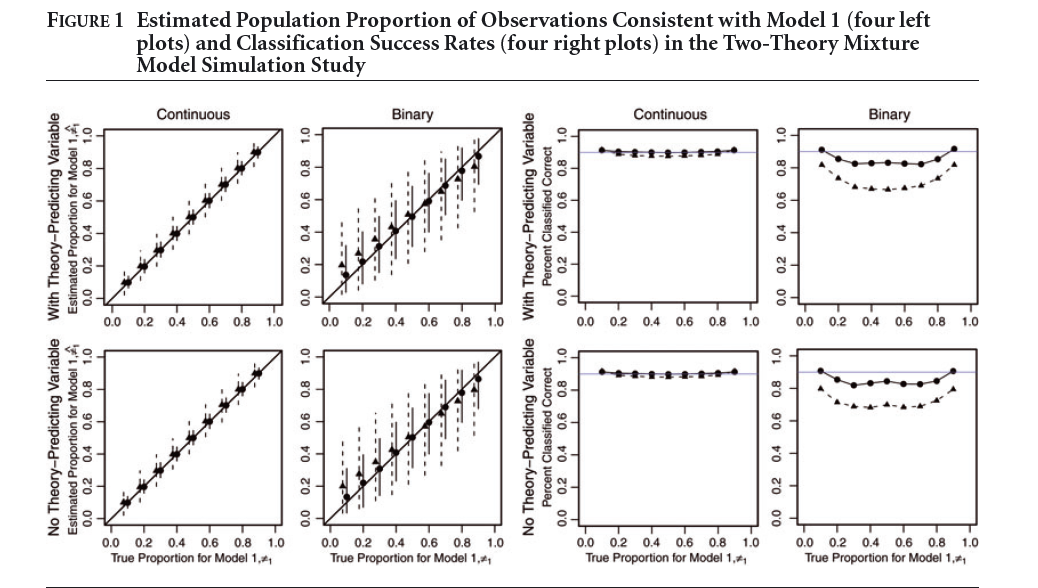
\includegraphics[width=0.7\linewidth]{theory_testing_sims}
	\caption{Testing Theory Testing with Simulations}
	
	\textit{Source:} Imai and Tingley (2012), pg. 228
	\label{fig:theory_testing_sims}
\end{figure}
\end{frame}                       


\begin{frame}
\frametitle{Empirical Tests: Ricardo-Viner vs Stolper-Samuelson}
\begin{figure}
	\centering
	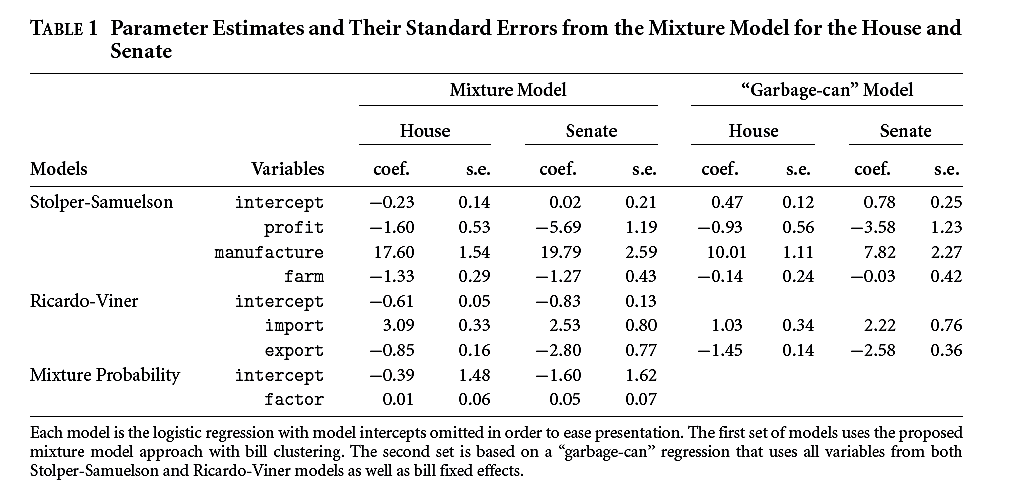
\includegraphics[width=0.7\linewidth]{table1}
	\caption{Coefficients for Trade Preference Models}
	
	\textit{Source:} Imai and Tingley (2012), pg. 232
	\label{fig:table1}
\end{figure}
\end{frame}

\begin{frame}
\frametitle{Empirical Tests: Ricardo-Viner vs Stolper-Samuelson}
\begin{figure}
	\centering
	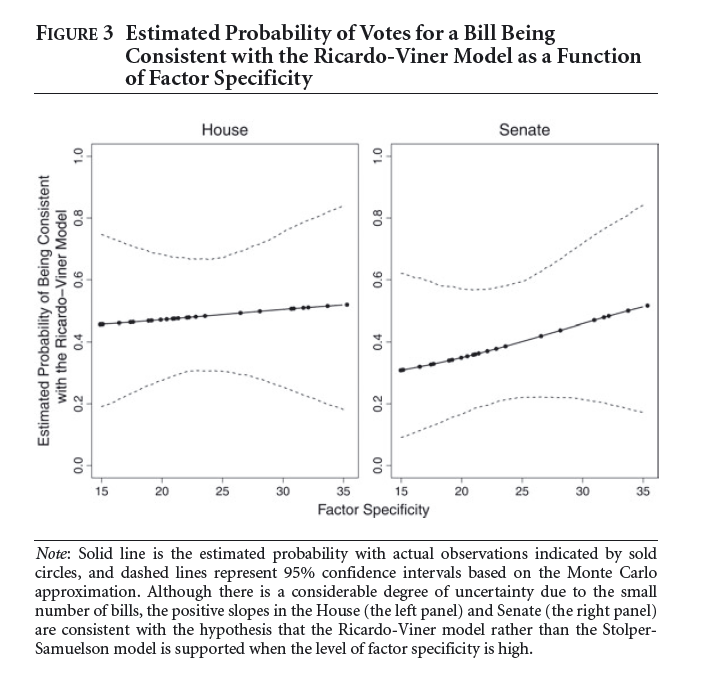
\includegraphics[width=0.7\linewidth]{rv_vs_ss}
	\caption{Theory Predicting Variable}
	
	\textit{Source:} Imai and Tingley (2012), pg. 231
	\label{fig:rv_vs_ss}
\end{figure}
\end{frame}     

\begin{frame}
\frametitle{Empirical Tests: Democratic Peace}
\begin{figure}
	\centering
	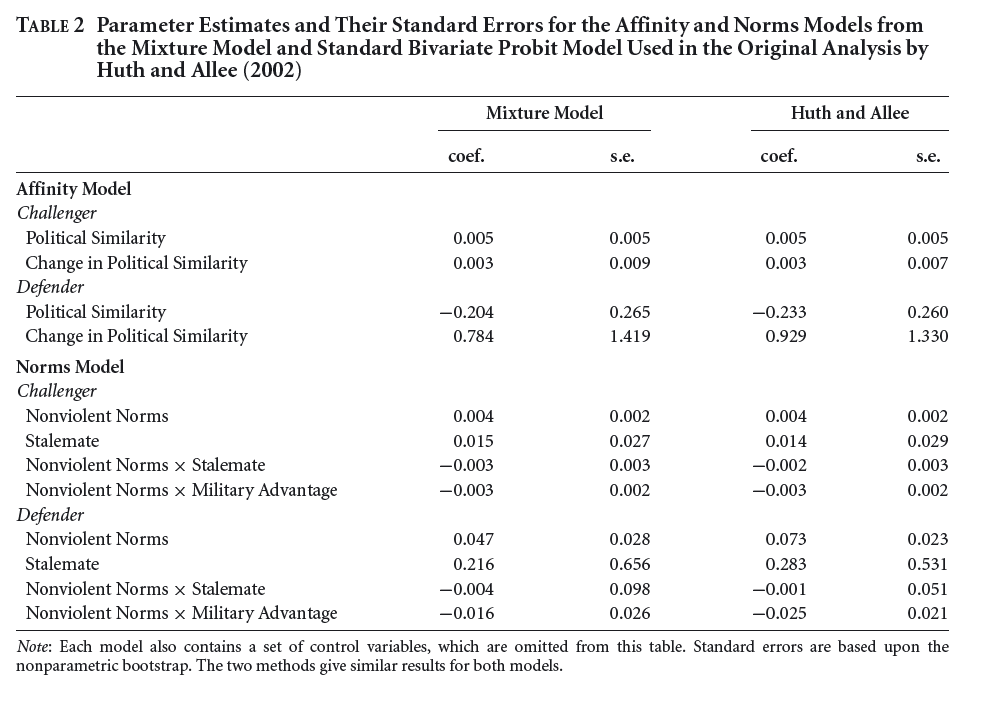
\includegraphics[width=0.7\linewidth]{table2}
	\caption{Democratic Peace Theories Coefficients}
	
	\textit{Source:} Imai and Tingley (2012), pg. 234
	\label{fig:table2}
\end{figure}
\end{frame}

\begin{frame}
\frametitle{Empirical Tests: Democratic Peace}
\begin{figure}
	\centering
	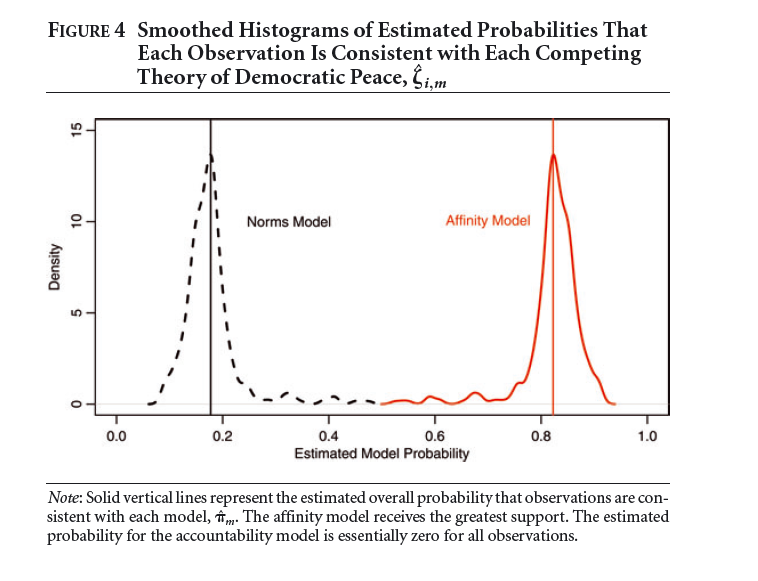
\includegraphics[width=0.7\linewidth]{figure4_dem_peace}
	\caption{}
	
	\textit{Source:} Imai and Tingley (2012), pg. 233
	\label{fig:figure4_dem_peace}
\end{figure}
\end{frame}

\begin{frame}
\frametitle{Discussion Questions}
\begin{enumerate}
	\item What is the difference between predictive and causal inference and why is it important for this paper? Why is it important for machine learning?
	\item What is one of the key differences in terms of assumptions between the finite mixture model approach and other, more traditional model selection approaches?
	\item How is this different from Bayesian model averaging?
	\item What are some of the limitations of this approach? 
	\item Under what conditions do you think it would be appropriate to think a theory produces one observation deterministically?
	\item What are some alternatives to model selection that Imai and Tingley did not discuss?
	\item How convincing do you find their empirical tests---the Ricardo-Viner vs Stolper-Samuelson theories of trade policy preferences and the three theories of the democratic peace?
\end{enumerate}
\end{frame}

\begin{frame}
\frametitle{Limitations}
\begin{itemize}
	\item Only helps with predictive inference, not causal inference
	\item Approach breaks down when you try to compare too many theories (Imai and Tingley recommend using two to three)
	\item Could be identification issues across the full model that aren't there in submodels
	\item High correlations across predictors are possible, which can impact power
	\item It is possible for a theory with more predictors to be selected purely because it has more predictors---it is very important to build and specify carefully, based in theory.
	\item It can be difficult to find \textit{theory-predicting variables}. 
\end{itemize}
\end{frame}



\begin{frame}
\frametitle{$J$ Test}
\begin{align}
Y_i = (1-\pi)f(X_i, \boldsymbol{\beta}) + \pi g(X_i, \boldsymbol{\gamma}) + \boldsymbol{\epsilon}_i
\end{align}
\end{frame}

\end{document}